\chapter{Psi}
%TODO Die Introduction fängt gut an, aber MicroPsi fällt mir zu sehr vom Himmel. Du solltest in der Introduction wirklich nur motivierend bleiben, warum will man so was wie MicroPsi haben, warum braucht man Simulationsumgebungen, keine Details zur MicroPsi-Implementierung oder Minecraft. Das kommt erst im Kapitel Foundations (dort kannst du den Text wahrscheinlich ziemlich so bringen, wie er in der Motivation steht)!

A widely accepted definition of the field of AI is that it is the study and design of intelligent agents, where an intelligent agent is a system that perceives its environment and takes actions that maximise its chances of success. %TODO find original sources

It took many years for AI research to evolve from the early ideas of thinking machines over Deep Blue, the computer that could beat mankind's best chess players to Watson, the AI that beats the champions of Jeopardy, the game show, that is about asking the appropriate question to a given answer. There exist many applications for AI~. Self-driving cars and online-shopping recommendation systems to name a few.

These examples have one thing in common. They are applications of technology that serves an immediate, or at least foreseeable purpose. For AI in scenarios of this kind, the term applied AI (or weak AI) has been coined.

Strong AI, in contrast, is about researching the nature of intelligence itself. An actual (hypothetical) implementation of a Strong AI translates to building a machine, that is capable of acting like a human being --- not just in a defined problem fields, but in all of them.

Putting it differently, weak AI considers computers to be an instrument to research cognitive processes. Strong AI considers simulated cognitive processes as actually being actual cognition. 

Cognitive AI, in particular, can be thought of as architectures that implement findings and theories in the fields cognitive science and psychology, as well as the neuro-sciences, for the sake of proving, if the theories hold against what they promise. 



Another term that is being used more and more is AIG for Artificial General Intelligence. It delimits itself from narrow AI applications, which chess would be an excellent example for. AIG sets out, to develop software, that can solve and act appropriately in a variety of problem fields, without specialising on any particular problem whatsoever. A complete AIG system is supposed to control itself autonomously and to have it's own thoughts and feelings. This has been the original focus of the AI field, before many lost their enthusiasm about it, because it turned out to be quite difficult. Even though the advances in narrow AI contribute also to AIG, AIG is more than just a collection of those. Many different AIG projects are in the making, with most of them being in early stages.\cite{goertzel2007artificial}

%... Examples for cognitive architectures are ...

Many cognitive architectures share characteristics with or directly implement artificial neural node nets.

Trying to figure out, if machines are able to implement cognition, we often explain it by enumerating the things that computers can not to. They can not be kind, friendly or have a sense of humor. Neither can they tell right from wrong, fall in love or learn from experience. But what can computers do? They are at least in parts involved in significant discoveries in most sciences. They steer cars safer than humanity ever did? Where, exactly, to put the dividing line?~\cite{russell2009artificial}

Looking upon the field of AI from a philosophical point of view, computers seem to deliver enormous potential for learning about how minds work. At the same time, new questions arise. If we would know how minds work, and if we could build machines that simulate cognition, would their minds be real? What would be the ethical implications? According to Russel and Norvig (in \cite{russell2009artificial}), one can differentiate in between two assumptions. The assertion, that computers are able to act \emph{as if} they were intelligent, is called the weak AI hypothesis. Thinking that an intelligently acting machine in fact \emph{is} performing cognition, is called strong AI hypothesis. What we believe is possible and what is not, becomes obsolete, once we are able to build something, that cognition can not be denied from. As Dijkstra put it: ``The question of whether Machines Can Think... is about as relevant as the question of whether Submarines Can Swim.''

The most famous indicator for whether a machine is intelligent or not, is the turing test. Decades after it's formulation, associated contests are still being held. May the best conversationalist win! Many would argue, that even and algorithm that passes the turing test, would still not be intelligent. It would trick people into thinking it was, but it would still not be conscious, aware of itself. Moreover, it would not have emotions. Dietrich Dörner thinks about it differently.~\cite{russell2009artificial}



\cite{russell2009artificial}

%... Approaches to cognitive AI ...
%... neural node nets ...
%... related work ...

\section{Psi Theory}
The Psi theory in its foundations was described by german psychologist Dietrich Dörner in his books ``Bauplan für eine Seele'' and ``Die Mechanik des Seelenwagens'' from 1998 and 2002. Dörners holistic approach goes beyond classic problem solving but develops a unified model for cognition that implements motivation and emotions. He is convinced, that artificial intelligence does not have to focus on different aspects of cognition that have to be looked at separately, but that a unified theory will eventually lead to a deeper understanding of cognition itself.

It's main ideas are, that it thinks of cognition as a graph-like structure (e.g. node-net) of relationships that strives to maintain homeostatic balance.\cite{Bach:2009:PSI:1611304}

Basic components of the theory are Representation, Memory, Perception, Drives, Cognitive modulation and emotion, Motivation, Learning and Problem solving as well as Language and consciousness. %(wikipedia)

"The basic conceptual element, analogous to Dietrich Dörner’s Psi theory, is the Quad. It makes use of a single ‘gen’ slot and the four directional gates ‘por’, ‘ret’, ‘sub’, ‘sur’. ‘Por’ encodes succession, ‘ret’ predecession, ‘sub’ a part-of relationship, and ‘sur’ stands for has-part. With the ‘gen’ gate, associative relationships can be expressed."

%... Basics of Psi Theorie of Dörner ...

Joscha Bach adapted that theory to bring it in a contemporary from with slight modifications in ``Principles of Synthetic Intelligence PSI: An Architecture of Motivated Cognition''~\cite{Bach:2009:PSI:1611304}.

Simulated environments proved to especially serve well in terms of researching collaborative behaviour of multiple agents, in terms of mapping and exploration, image procecessing as well as memory and planning. Additionally, some scenarios are almost impossible to implement in the physical world, as evolving agent populations, for example. On the other hand, downsides of simulated worlds include them being limited by computing power and the programmer's specifications.
MicroPsi provided a simulation component with a server for objects in three dimensional space
most experiments take place on a plane
ground types bitmap
basic administrator interface
clickable objects
3D view
predefined island as well as mars

mars und island screens
objects may be made up recursively of subobjects
objects have classes
DirectX based 3D world viewer

\cite{Bach:2009:PSI:1611304}

%... explanation of Joschas Dissertation ...

%\section{Summary}
Even though building a conscious machine that thinks and acts like we do is still mere science-fiction, it is this kind of foundational research, that leads no new ways of thinking of the world, that give us our most import leaps.

%... still a lot to do in AI ...

    \section{Psi Implementations}
Psi has been implemented by different groups at different times. The first implementations are by Dörner and his associates themselves~(see figure \ref{psi_screen}). They used Pascal and developed it for Windows environments. This implementation can still be downloaded and runs on Windows 7 installations, for example.

\begin{figure}[h]
  \centering
    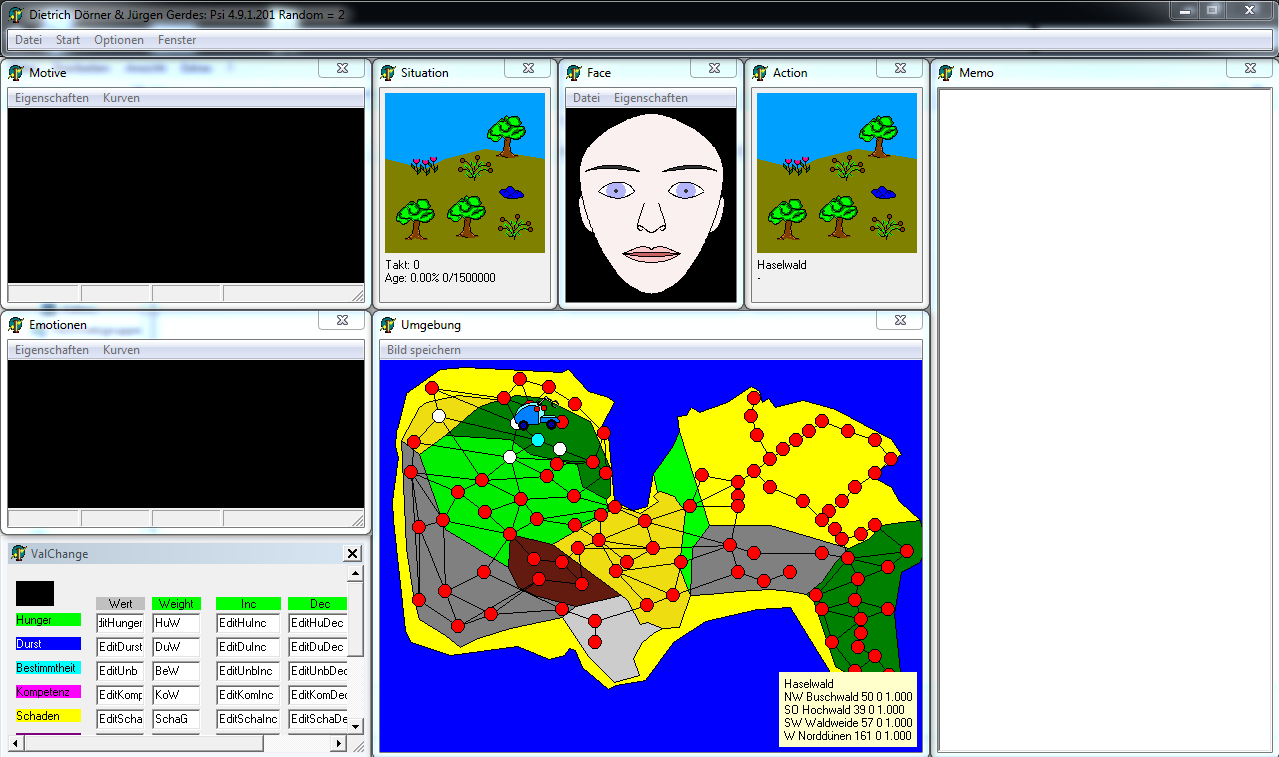
\includegraphics[width=10cm]{graphics/psi_screen1}
  \caption{Dörner's Pascal Psi Implementation}
  \label{psi_screen}
\end{figure}

The work on Dörner's team's implementation has not been continued, so Joscha Bach and his associates built new implementations of Psi.

From 2003 to 2009 they built an implementation in Java as a set of plugins for the Eclipse IDE called MicroPsi. It included a graphical editor and a 3D simulation-environment. 

    \section{MicroPsi 2}
Aiming at better understandability and to maintain platform independence, MicroPsi has been built ground up again in 2011 and 2012 using more lightweight Python code. What is remarkable about the new implementation called MicroPsi 2 (in the following MicroPsi), is that the simulation is deployed as a web application and the graphical interface is completely rendered inside a web browser using state-of-the-art internet- and webapplication-technologies.~\cite{conf/agi/Bach12}
        
Even though there have been more complex simulation environments (e.g. 3D-worlds) for previous implementations of Psi-architectures, the relatively new version of MicroPsi has only two fairly simple ones: a 2D-Island and a map of the public transportation system of Berlin~(see figure~\ref{mp2_berlin}). Instead of building a new 3D-world, with this project we set out for something more experimental. More on this in chapter three and four.

\begin{figure}[h]
  \centering
    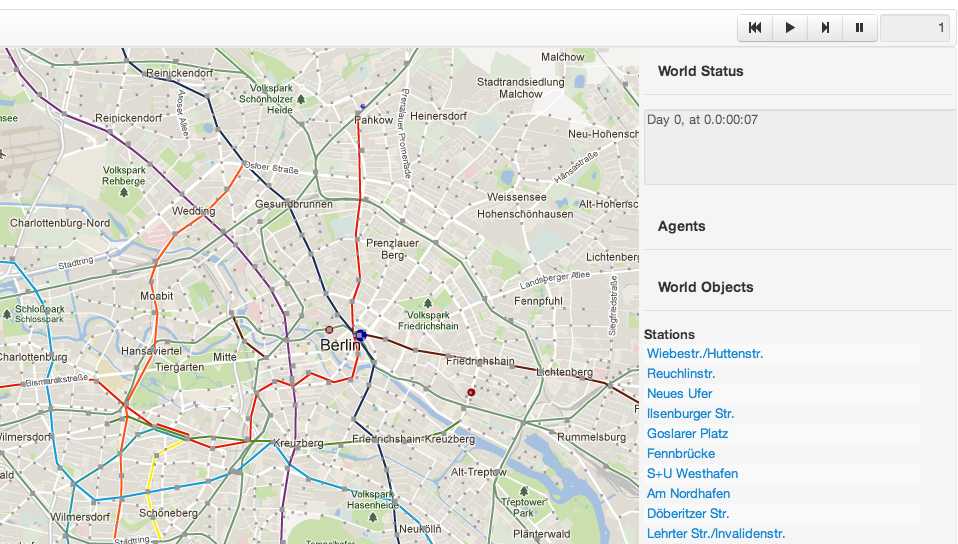
\includegraphics[width=10cm]{graphics/mp2_berlin}
  \caption{MicroPsi simulation environment Berlin}
  \label{mp2_berlin}
\end{figure}

        \subsection{Module Overview}
MicroPsi is written in Python with a minimum of dependencies. Therefore its  modular structure is comparably easy to understand. It is illustrated in figure~\ref{micropsi2_modules}. First, one can differentiate in between the \texttt{Server} module (or the web-interface) and the actual simulation \texttt{Runtime} module (also called ``core''). In a regular simulation experiment setup, MicroPsi runs three threads: one for the \texttt{Server} and, invoked by the \texttt{Runtime}, one \emph{world runner} that runs a simulation world as well as one \emph{node net runner} that runs the node net. As these names suggest, the \texttt{Runtime} manages both the simulations environments as well as the inhabitant agents (or node net embodiments). They may by design run asynchronously. In fact, the \texttt{Runtime} works entirely independent of the \texttt{Server} and therefore may just as well be deployed for command line interaction or other GUIs. Furthermore, the \texttt{Server} contains a \texttt{UserManager} and the \texttt{Runtime} a \texttt{ConfigurationManager}.~\cite{conf/agi/Bach12}
\\          
          
\begin{figure}[h]
  \centering
    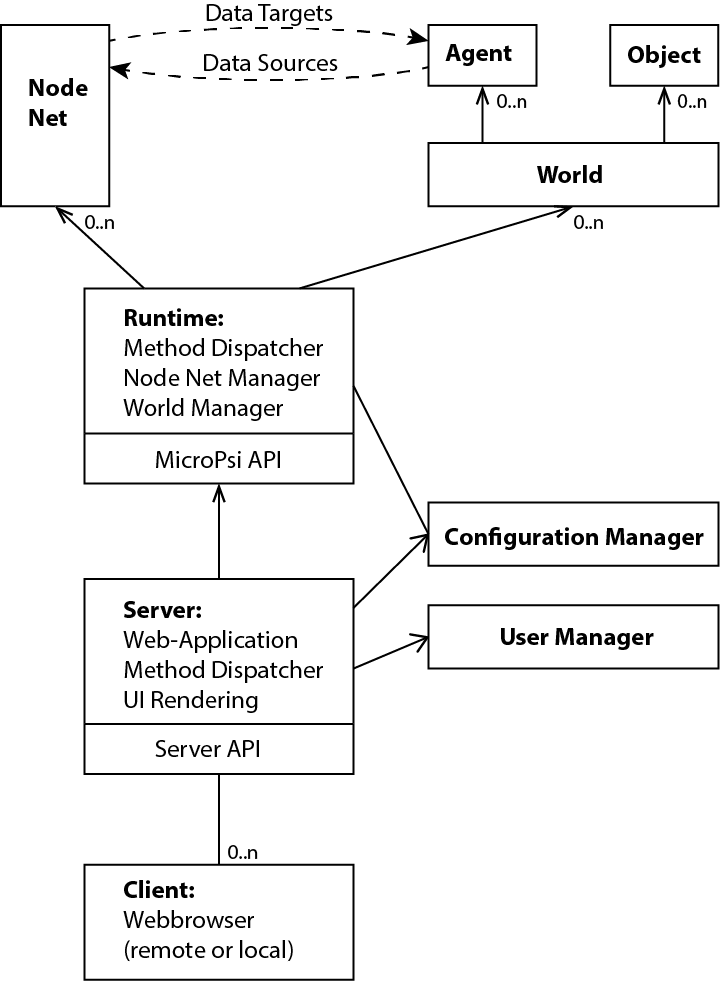
\includegraphics[width=8cm]{graphics/micropsi2_uml}
  \caption{The modular architecture of the MicroPsi framework make it easy to extend. (taken from~\cite{conf/agi/Bach12})}
  \label{micropsi2_modules}
\end{figure}

The following description is heavily based on \cite{conf/agi/Bach12}, where the theoretical foundations can be found in detail.

        \subsection{Module \texttt{Server}}
The \texttt{Server} renders the GUI and deploys the agent simulation as a web application. It acts as a \emph{web server} for remote or local access. A client for this application may be any computer with a reasonable up-to-date web browser. Therefore simulations can be launched from anywhere without requiring any installation. It rests upon the lightweight Python web framework \emph{Bottle}.

The web interface is naturally based on HTML as well as Javascript. The communication in between the browser and the simulation is managed via JSON remote procedure calls. Many GUI components of Twitter's \emph{Bootstrap} library are in use. The graphic renderings (see figure~\ref{micropsi2_nodenet}) utilise the JavaScript graphics library \emph{PaperJS}. 

\begin{figure}[h]
  \centering
    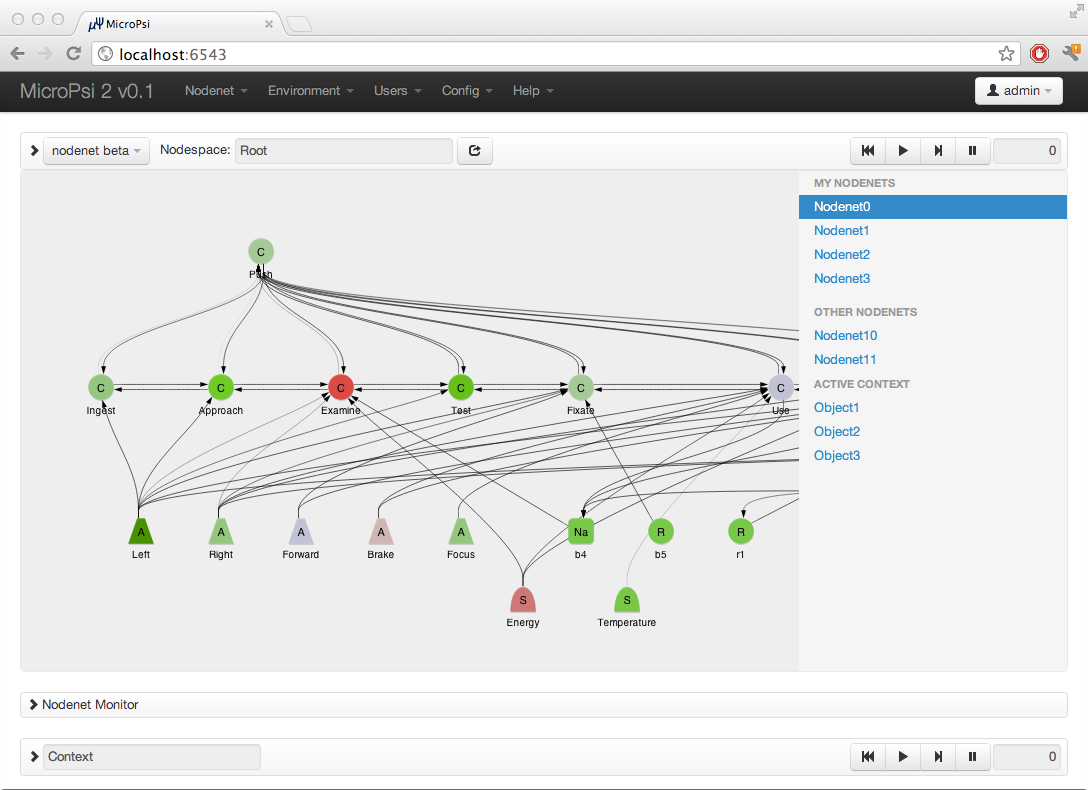
\includegraphics[width=8cm]{graphics/micropsi2_nodenet}
  \caption{The graphical editor is the primary interface to node nets. (taken from~\cite{conf/agi/Bach12})}
  \label{micropsi2_nodenet}
\end{figure}

The \texttt{Server} communicates with its users through the server API. User sessions and access rights are managed by the \texttt{UserManager}.
   
        \subsection{Module \texttt{Runtime}}
In this setup, the \texttt{Server} starts the \texttt{Runtime} --- even though it may also work independently of the \texttt{Server}. The \texttt{Runtime} component communicates with the \texttt{Server} through the MicroPsi API. It manages node nets and worlds.

        \subsubsection{Node Nets}
A MicroPsi node net is defined as a set of states, a starting state, a network function, ``that determines how to advance to the next state'' and a set of node types. Data sources and data targets serve as input and output towards a world, where a data source is filled with data from the world and data targets are linked to agent actions in the world.

According to the Psi theory, nodes may have different types and parameters. They contain gates and slots that send and receive activation. In most cases, the activation is forwarded from a slot to a gate without further modulation.

Nevertheless, nodes may contain functions that enable the creation of new nodes and links as well as procedures for learning and planning. They may be implemented as Python code.

According to the concepts of the Psi Theory, MicroPsi defines agents as node nets or, to be more specific, hierarchical spreading activation networks. They are an "abstraction of the information processing provided by brains"~\cite{conf/agi/Bach12}. Agents can be placed and researched in simulation environments or physically embodied as robots.

As node nets share the relevant characteristics with neural node nets, they may enable neural learning paradigms. To store information they can form semantic networks. Furthermore, nodes may contain state machines and other operations, which make it possible to build modularised architectures.

        \subsubsection{Worlds}
The simulations worlds are the environments in which we can study our agent's behaviour. Worlds need to provide a world adapter which functions as the interface in between a node net and the environment. Within the world adapter data sources and data targets have to be defined carefully, to get a functional and meaningful experiment going. They represent the agent's sensory input and motoric output. Sophisticated interconnection of those enables interaction with the environment.

The kind of data the world adapter interfaces, is not specified any further, which gives developers the opportunity to experiment with classic simulation worlds as well as exotic applications (eg. stock data). At the time of the original development of the framework, the priorised application was building a framework for knowledge representation.

        \paragraph{Objects}$\;$ \\
Worlds contain objects. Objects may be anything that could be interesting for a simulation and that needs some kind of integrated logic. Light sources or collectable resources are a common example. Objects may contain a set of functions and states, but at least one function that determines how the object advances and reacts to changes while moving through a simulation cycle. 

A comprehensive world functions calls every object function for each simulation step of the world.

        \paragraph{Agents}$\;$ \\
Agents are objects that are connected to a world adapter which makes them controllable by a node net. The object that incarnates the agent is best thought of as the agents body. The function that advances the object checks for input from the node net and outputs to it.
        